\documentclass{article} 
\usepackage{amsmath}
\usepackage{amssymb}
\usepackage{graphicx}
\usepackage{fancyhdr}
\pagestyle{fancy}
\lhead{} 
\chead{} 
\lhead{\bfseries Group: SHPZKN}
\rhead{\bfseries ML Homework 6} 

\newcommand{\Lagr}{\mathcal{L}}
\newcommand{\R}{\mathbb{R}}

\begin{document}
\section{Problem 1}
%%% a--------------------------------------------------------------------------------------------------------------------------------
%a)\\
%We know the general formula on the below, and we want to apply two vector to $X$ and $Y$,
%find out the maximum value of correlation coefficient.
%\begin{flalign*}
%\begin{split}
%Corr(X,Y) &= \frac{Cov(X,Y)}{\sqrt{ Var(X)Var(Y)}}\\
%&=\frac{w_x ^\intercal Cov(X,Y) w_y}{\sqrt{w_x^\intercal Var(X) w_xw_y^\intercal Var(Y) w_y}}
%\end{split}&
%\end{flalign*}
%%%% b----------------------------------------------------------------------------------------------------------------------------------
%b)\\
%We use different notion of covariance ($\Sigma$) in the answer.
%\begin{flalign*}
%\begin{split}
%\rho = \frac{w_x ^\intercal \Sigma_xy w_y}{\sqrt{w_x^\intercal \Sigma_xx w_xw_y^\intercal \Sigma_yy w_y}}\\
%%Maximazing the covariance between x and y is same as maximazing the correlation. we set the constriction\\
%w_x^\intercal \Sigma_xx w_x =1\\
%w_y^\intercal \Sigma_yy w_y = 1
%\end{split}&
%\end{flalign*}

\section{Problem 2}
%%% a--------------------------------------------------------------------------------------------------------------------------------
a)\\
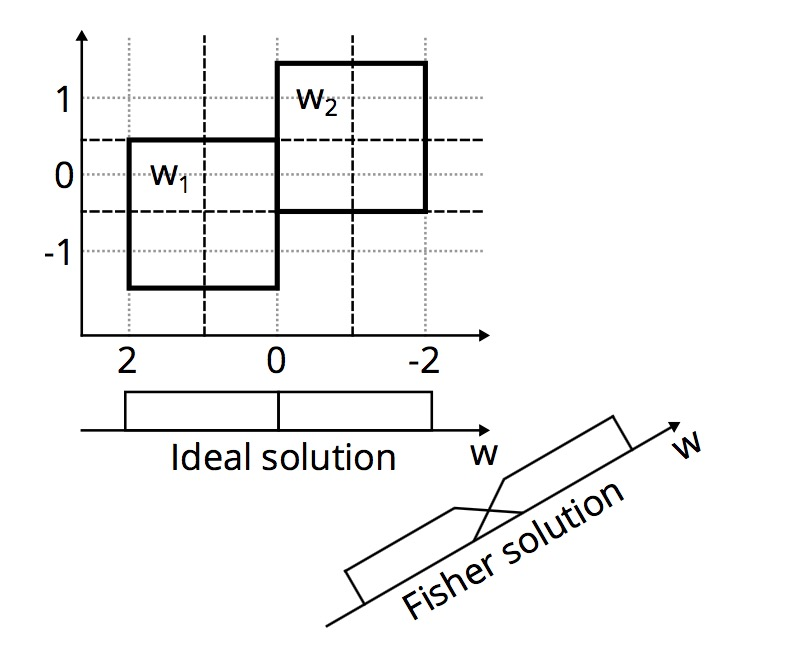
\includegraphics[width=12cm, height=8cm]{hm6.jpg}
\\
Consider two distributions $p(x|w_1)\sim U(a,b)^2 = U(-1,1)^2$ and $p(x|w_2) \sim U(-1,1)^2$, then we define the expectation as:
\begin{equation*}
\mu_1=\begin{pmatrix}
         -1 \\
         -0.5 
        \end{pmatrix}
        \qquad \text{and} \qquad
\mu_2 = \begin{pmatrix}
         1 \\
         0.5 
        \end{pmatrix}
\end{equation*}
We define $X$ as a random variable for first dimension, $Y$ as a random variable for second dimension, and we assume, that two variables are iid. So, we can say, $Cov(X,Y)=Cov(Y,X) = 0$, therefore, we know the variance of $X$ and $Y$, $Var(X) = Var(Y) = \frac{1}{12}(a-b)^2 = \frac{1}{3}$, The covariance matrix is on the below.
\begin{equation*}
\Sigma= \begin{bmatrix}
         Var(X) & Cov(X,Y)\\
         Cov(Y,X) &Var(Y)
        \end{bmatrix}
        = \begin{bmatrix}
        \frac{1}{3} & 0\\
        0& \frac{1}{3}
        \end{bmatrix}
        = \frac{1}{3}I
\end{equation*}
We can compute $w^*$:
\begin{equation*}
w^* = \Sigma_w^{-1}(\mu_2-\mu_1) 
\Sigma= 3I\begin{pmatrix}
                     \begin{pmatrix}
                     1\\
                     0.5
                     \end{pmatrix} -
                      \begin{pmatrix}
                     -1\\
                     -0.5
                     \end{pmatrix}
                \end{pmatrix} 
             = 3 \begin{pmatrix}
                     2\\
                     1
                     \end{pmatrix}  
             \neq  \begin{pmatrix}
                     1\\
                     0
                     \end{pmatrix} 
\end{equation*}
where $\begin{pmatrix}
                     1\\
                     0
                     \end{pmatrix} $ would be the optimal Bayes solution (from the pic). The linear prediction in Bayes can easily obtained by $p(w_1|x)>p(w_2|x)$, which is different with Fisher discriminant analysis.
 \\  
 \\                  
%%% b--------------------------------------------------------------------------------------------------------------------------------    
b)\\
When the two classes are generated by two d-dimensional Gaussian distributions,
\begin{flalign*}
\begin{split}
p(x|w_1) &= \frac{1}{\sqrt{2\pi det(\Sigma_1)}}exp \left(-\frac{1}{2}(x-\mu_1)^ \intercal \Sigma_1^{-1}(x-\mu_1) \right)\\
p(x|w_2) &= \frac{1}{\sqrt{2\pi det(\Sigma_2)}}exp \left(-\frac{1}{2}(x-\mu_2)^ \intercal \Sigma_2^{-1}(x-\mu_2) \right)
\end{split}&
\end{flalign*}
According to question a, if we decide $w_1$, therefore,
\begin{flalign*}
\begin{split}
p(w_1|x)&>p(w_2|x)\\
\frac{p(x|w_1)p(w_1)}{p(x)}&>\frac{p(x|w_2)p(w_2)}{p(x)}\\
p(x|w_1)p(w_1) &>p(x|w_2)p(w_2)
\end{split}&
\end{flalign*}
where we take the logarithm to simplify the computation:
\begin{flalign*}
\begin{split}
\ln{p(x|w_1)} + \ln{p(w_1)} &> \ln{p(x|w_2)} + \ln{p(w_2)}\\
\ln{p(x|w_1)} -  \ln{p(x|w_2)} &> \ln{p(w_2)} - \ln{p(w_1)}\\
-\frac{1}{2}\ln{2\pi} -\frac{1}{2}\ln{det(\Sigma_1)} - \frac{1}{2}(x-\mu_1)^\intercal \Sigma_1^{-1}(x-\mu_1) &\\+\frac{1}{2}\ln{2\pi} +\frac{1}{2}\ln{det(\Sigma_2)} + \frac{1}{2}(x-\mu_2)^\intercal \Sigma_2^{-1}(x-\mu_2) &>
\ln{p(w_2)} - \ln{p(w_1)} 
\qquad \text{(PS: plug into above pdf)}
\end{split}&
\end{flalign*}
We can identify the first part of the inequality as the mapping $\phi: \R^d\rightarrow\R$
$$\phi(x) = (x-\mu_2)^\intercal \Sigma_2^{-1}(x-\mu_2) - (x-\mu_1)^\intercal \Sigma_1^{-1}(x-\mu_1)$$
which is the optimal solutions in Bayes sense.

\end{document}